%!TEX root = ../thesis.tex

\chapter{Artefacts in Optimal Extraction}
\label{appendix:artefacts}

%!TEX root = ../../thesis.tex
% Table of nods replaced for correction.
\change{Maybe transpose \cref{tab:nod_replacement} to be shorter?}{}
\change{CHANGE \# into the ESO identification number 1b 2a etc}
\begin{table}
    \caption{Identification of all the optimally reduced nod spectra which had artefacts that were replaced by the rectangular extractions, corrected for bad pixels. The numbers represent the position in the nod cycle ABBAABBA.\@The number of the observation for each target is given by \#.}
    \label{tab:nod_replacement}
    \centering
    \begin{tabular}{cccccccc}
        \toprule
      & & \multicolumn{4}{c}{Detector}& \\
         Target  & \#  & 1 & 2 & 3 & 4 & Total \\
        \midrule
        \object{HD 4747}   & 1 & 8 & 5, 8 & 8 & 1, 5, 8 & 7\\
        \object{HD 162020} & 1 & - & 7, 8& - & - & 2\\
        \object{HD 162020} & 2 & - & 2 & - & 8 & 2\\
        \object{HD 167665} & 1 & 2, 4 & 8 & 1, 6 &  4, 5 & 7\\
        \object{HD 167665} & 2 & 2 & 3 & 1 & 8 & 4\\
        \object{HD 167665} & 3 & 6 & 3, 7 & - & 8 & 4\\
        \object{HD 168443} & 1& - & - & - & 7, 8 & 2\\
        \object{HD 168443} & 2 & - & 2, 4 & 6 & 8 & 4\\
        \object{HD 202206} & 1 & - & 6, 7& 1& - & 3\\
        \object{HD 202206} & 2 & 5 & - & 7,8 & - & 3\\
        \object{HD 202206} & 3 & 8 & 3 &  6 & 6 & 4\\
        \object{HD 211847} & 1 & - & 5, 7 & 2 & 4 & 4\\
        \object{HD 211847} & 2 & 2 & 1, 7 & 7 & 8 & 5\\
        \object{HD 30501}  & 1 & 7 & 7 & - & 8 & 3\\
        \object{HD 30501}  & 2 & 7, 8 & 3, 5, 7, 8 & 2, 7 & 2, 3&10 \\
        \object{HD 30501}  & 3 & 4, 8 & 2, 6, 7& 4, 8 & 7& 8\\
        \object{HD 30501}  & 4 & 1, 2, 4 & 3 & 5, 6 & 6 & 7\\
         \midrule
            &&16&27&17&19& 79/544\\
    \bottomrule
    \end{tabular}
\end{table}


%!TEX root = ../../thesis.tex
% Tally nods replaced for correction.
\begin{table}
    \centering
    \caption{Tally of nod cycle positions in which their optimally reduced spectra were affected and were replaced.}
    \begin{tabular}{lccccccccr}
        \toprule
        Order Number & 1 & 2 & 3 & 4 & 5 & 6 & 7 & 8 &Total\\
        Nod Position & A & B & B & A & A & B & B & A & \\
        \midrule
        Tally & 6 & 10 & 6 & 7 & 7 & 9 & 15 & 19 & 79\\
        \bottomrule
    \end{tabular}\label{tab:nod_artefact_tally}
\end{table}

\begin{figure}
    \centering
    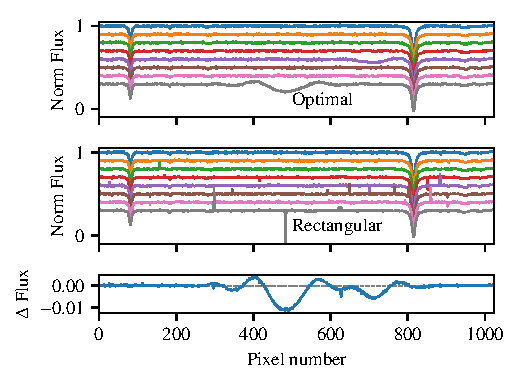
\includegraphics[width=0.7\linewidth]{figures/appendix/bp_plots/extraction_comparision_HD4747-1_chip_2}
    \caption[]{Artefact example for the second detector of {HD\,4747}.
        The top panel contains the eight normalized nod spectra obtained using optimal extraction.
        The middle panel shows nod spectra using only rectangular extraction.
        The bottom panel shows the difference between a combined spectrum using optimal nods only and a combined spectrum in which the identified nods are replaced with their rectangular counterparts as per \cref{subsubsec:reductionartefacts}.
        A vertical offset is included between each spectra for clarity.
        The nod spectra are in observation order from top to bottom.
        In this example there are artefacts in the \nth{5} (purple) and eighth (grey) nod spectra around 700 and 500 pixels respectively.}
    \label{fig:artefact_example1}
\end{figure}
\begin{figure}
    \centering
    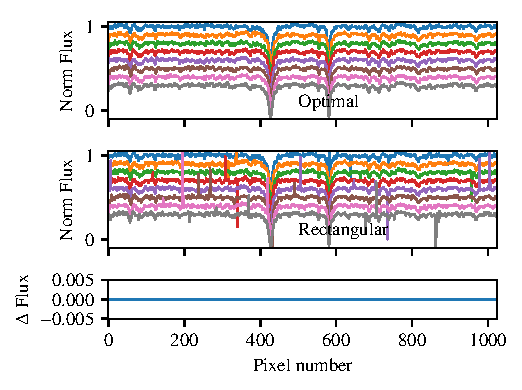
\includegraphics[width=0.7\linewidth]{figures/appendix/bp_plots/rescaled_extraction_comparision_HD162020-2_chip_1}
    \caption[]{Same as \cref{fig:artefact_example1} but for the first detector of the second observation of {HD\,162020}.
        In this example there are several large spikes observed in the rectangular extraction but they do not appear to effect the optimally extracted nods (there are no artefacts).}
    \label{fig:artefact_example2}
\end{figure}
\begin{figure}
    \centering
    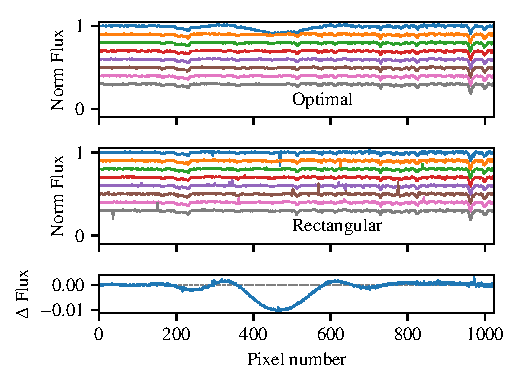
\includegraphics[width=0.7\linewidth]{figures/appendix/bp_plots/extraction_comparision_HD167665-1b_chip_3}
    \caption[]{Same as \cref{fig:artefact_example1} but for the third detector of the second observation of {HD\,167665}.
        In this example a small spike in the first spectrum (blue) around pixel 450 causes an extended dip in the optimally extracted nod.}
    \label{fig:artefact_example3}
\end{figure}
\begin{figure}
    \centering
    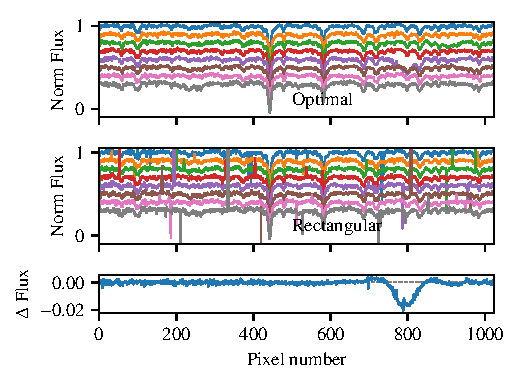
\includegraphics[width=0.7\linewidth]{figures/appendix/bp_plots/extraction_comparision_HD202206-2_chip_1}
    \caption[]{Same as \cref{fig:artefact_example1} but for the \nth{1} detector of the second observation of {HD\,202206}.
        In this example there are several large spikes but only one produces an artefact.
        This is on the \nth{5} nod (purple) around pixel 800.}
    \label{fig:artefact_example4}
\end{figure}
\begin{figure}
    \centering
    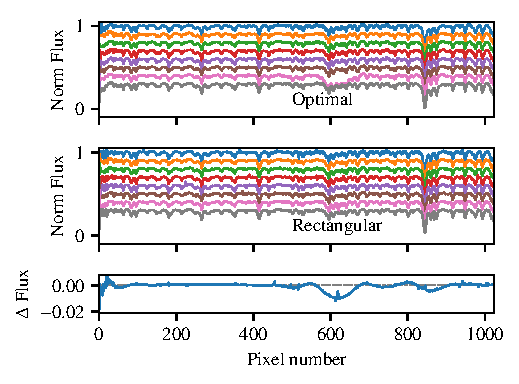
\includegraphics[width=0.7\linewidth]{figures/appendix/bp_plots/extraction_comparision_HD168443-1_chip_4}
    \caption[]{Same as \cref{fig:artefact_example1} but for the fourth detector of the first observation of {HD\,168443}.
        In this example a barely visible spike on the  \nth{7} nod (pink) causes a deviation in the optimal nod around pixel 610.
        There is also a second small spike on the eighth nod (grey) around pixel 850, between two spectral lines.}
    \label{fig:artefact_example5}
\end{figure}
\begin{figure}
    \centering
    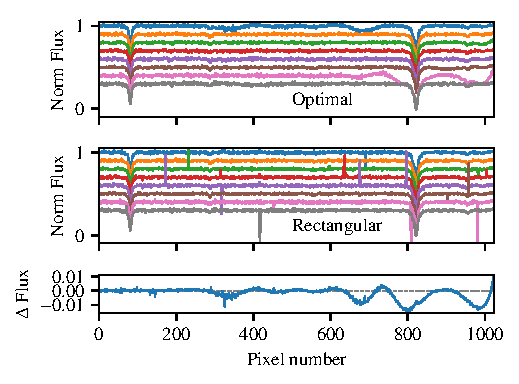
\includegraphics[width=0.7\linewidth]{figures/appendix/bp_plots/extraction_comparision_HD211847-2_chip_2}
    \caption[]{Same as \cref{fig:artefact_example1} but for the second detector of the second observation of {HD\,211847}.
        In this example two large spikes around 800 and 1000 in the \nth{7} nod (pink) create large deviations in the optimally reduced spectra.
        A spike in the first nod (blue) around pixel 700 also causes a bump.
        There is also some extra noise in the first nod around pixel 350.}
    \label{fig:artefact_example6}
\end{figure}
\begin{figure}
    \centering
    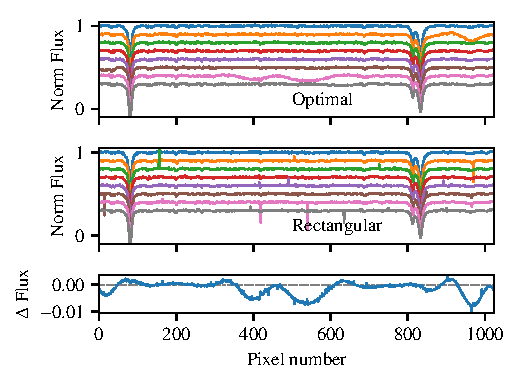
\includegraphics[width=0.7\linewidth]{figures/appendix/bp_plots/extraction_comparision_HD30501-2b_chip_2}
    \caption[]{Same as \cref{fig:artefact_example1} but for the second detector of the second observation of {HD\,30501}.
        In this example there are artefact causing spikes in four places.
        The second nod (orange) around pixel 950, the \nth{6} nod (brown) around pixel 20 and two spikes in the \nth{7} nod (pink) around pixels 400 and 550.}
    \label{fig:artefact_example7}
\end{figure}

As mentioned in \cref{subsubsec:reductionartefacts} there were several artefacts observed in the \emph{optimal} reduction of the {DRACS} pipeline, coinciding with spikes in the \emph{rectangular} reduction.
A list of all specific nods of each observation and detector that were observed to contain artefacts and were replaced with the method developed are provided in \cref{tab:nod_replacement}.

With 8 nods per observation, and 4 {CRIRES} detectors for the 17 observations there are 544 individual nod spectra.
\Cref{tab:nod_replacement} identifies the 79 individual nods (14.5\%) that were found to contain artefacts while \cref{tab:nod_artefact_tally} provides a tally of the frequency of artefacts occurring within each nod position of the nod cycle.
Only 16/68 (23.5\%) detector-observations have all nods without any artefacts while no observation is completely free of artefacts across all 4 detectors.

Tallying the number of artefacts that occur per detector and nod position reveals three main features. The first is that there are around 1.3-1.5$\times$ more artefacts that occur on the second detector compared to the other three detectors individually.
This may be due to a physical defect with this detector, such as the large scratch seen in \cref{fig:masterflats_colour}, or it is possibly due to the relatively featureless spectrum on the second detector.
Either will make it easier to visually detect artefacts in the spectra, or easier for artefacts to be created by the pipeline.
The second is that there are more artefacts in the seventh and eight nods with $\sim40$\% of the artefacts in the last 2/8 of observations (see \cref{tab:nod_artefact_tally}).
As the artefacts occurr later in the nod cycle this suggests that they may be related to the operation of the instrumentation, for which the probability is built up over the repeated nod cycle observations, however this is just speculation.

There does not seem to be a connection between the nod position as both position A and B have half of the artefacts.
There is a higher number of artefacts occurring in the last two nods, suggesting that there may be some correlation to the length of the observation.
The growth in artefacts over time is not linear with a rapid increase starting around the sixth nod.

The third thing that is noticed is the difference in the number of artefacts seen in the first observation of HD\,30501 compared to the other three.
This was observed four months before the others, which were observed within the same week.
The later three observation all have larger number of artefacts 2--3$\times$ compared to the first observation.

The ideas presented here are only observations and speculation on the causes.
Tests for statistical significance of the differences observed have not been performed and is beyond the scope of this work.

\Crefrange{fig:artefact_example1}{fig:artefact_example6} show more examples of observed spectra in which spikes and artefacts are observed.
One example is given for each target, selected to show a variety of the artefacts observed.

In each image the top panel contains the 8 nod spectra extracted using the optimal method, which includes variance weighting.
The middle panel contains the rectangular extraction only (no variance weighting), The bottom panel shows the difference between the average combined spectra from the top and middle panels.

It is clear that the large extracted artefacts occur due to single spikes observed in the rectangular extraction.
What is unclear is the other factors that affect their cause.
For example in \cref{fig:artefact_example2} several spikes are seen but no artefacts are created.

% Add to list of figures.
\addtocontents{lof}{\protect\contentsline{figure}{\ref{fig:artefact_example1}--\ref{fig:artefact_example7} \quad {\color{hrefurlcolor} Extra examples of reduced spectra with artefact. One for each target.}}{{\color{black}\pageref{fig:artefact_example1}}}{}}
